\documentclass[11pt]{article}

% Use review mode for submission, change to final for camera-ready
\usepackage[preprint]{acl}

% Standard packages
\usepackage{times}
\usepackage{latexsym}
\usepackage[T1]{fontenc}
\usepackage[utf8]{inputenc}
\usepackage{microtype}
\usepackage{inconsolata}

% Additional packages
\usepackage{graphicx}
\usepackage{booktabs}

% Packages for methodology section (TikZ diagrams, algorithms, code listings)
\usepackage{tikz}
\usetikzlibrary{positioning, arrows.meta, shapes.geometric}
\usepackage{algorithm}
\usepackage{algpseudocode}
\usepackage{listings}
\usepackage{xcolor}
\lstset{
    basicstyle=\small\ttfamily,
    keywordstyle=\color{blue},
    commentstyle=\color{gray},
    stringstyle=\color{red},
    showstringspaces=false,
    breaklines=true,
    frame=single,
    numbers=left,
    numberstyle=\tiny\color{gray}
}
\IfFileExists{multirow.sty}{\usepackage{multirow}}{}
\usepackage{array}
\usepackage{url}
\usepackage{hyperref}
\usepackage{bookmark}

% Title and authors
\title{Architectures for Code Development with LLMs:\\ A Comparative Study of Multi-Agent Approaches}

\author{
  Riccardo Marconi \\
  Politecnico di Torino \\
  \small\texttt{riccardo.marconi@studenti.polito.it}
  \And
  Name Surname \\
  Politecnico di Torino \\
  \small\texttt{email@studenti.polito.it}
  \And
  Name Surname \\
  Politecnico di Torino \\
  \small\texttt{email@studenti.polito.it}
  \AND
  Name Surname \\
  Politecnico di Torino \\
  \small\texttt{email@studenti.polito.it}
  \And
  Name Surname \\
  Politecnico di Torino \\
  \small\texttt{email@studenti.polito.it}
}

\begin{document}
\maketitle

\begin{abstract}
  Large language models (LLMs) demonstrate impressive code generation capabilities, yet single-prompt interactions often fail on complex development tasks. We investigate whether multi-agent architectures improve code quality through role specialization and iterative refinement. We compare three approaches---Naive (one-shot generation), Single-Agent (5-stage pipeline with self-refinement), and Multi-Agent (Planner-Coder-Critic coordination)---across 25 programming tasks spanning five domains and three difficulty levels. Surprisingly, Multi-Agent and Naive achieve identical overall correctness (77.6\%), outperforming Single-Agent (74.6\%). However, Multi-Agent excels in algorithmically demanding domains (DSA: 85.9\%, Logic: 75.7\%) and medium-difficulty tasks (91.8\%), justifying its 20$\times$ computational overhead only for specific task types. Our findings reveal that architectural sophistication benefits complex algorithmic reasoning but can hurt performance on simple tasks through over-refinement.
\end{abstract}

\section{Introduction}

% TODO: Write introduction section
\textit{Large language models have revolutionized automated code generation, with models like Codex~\citep{chen2021evaluating} and Code Llama~\citep{roziere2023code} demonstrating remarkable capabilities. However, single-prompt approaches often struggle with complex development tasks requiring multi-step reasoning, systematic debugging, and quality assurance.}

\textit{Recent work in multi-agent systems~\citep{hong2023metagpt, qian2023chatdev} suggests that distributing responsibilities across specialized agents (e.g., planning, coding, reviewing) may improve software development outcomes. Yet, no systematic evaluation exists comparing single-agent and multi-agent architectures for code generation across diverse task types and complexity levels.}

\textit{This work addresses this gap through a controlled comparison of three architectural approaches on 25 programming tasks. Our key finding is that architectural sophistication does not uniformly improve performance---benefits are highly task-dependent, with multi-agent coordination excelling on algorithmic reasoning but struggling on simple pattern-matching tasks.}

\subsection{Research Questions}

We address the following research questions from the assignment requirements:

\begin{enumerate}
  \item \textbf{RQ1:} How do the architectures compare in terms of functional correctness and code quality?
  \item \textbf{RQ2:} How do agent coordination strategies impact correctness?
  \item \textbf{RQ3:} Does modular role separation improve code generation?
\end{enumerate}

\section{Background}

% TODO: Expand with more related work
\textit{Provide an overview of relevant work in the literature related to your task.}

\textbf{LLM-based Code Generation.} Early work on neural code generation~\citep{austin2021program} demonstrated feasibility of program synthesis from natural language. Recent code-specialized models like StarCoder~\citep{li2023starcoderbase}, CodeLlama~\citep{roziere2023code}, and Qwen2.5-Coder~\citep{qwen2024} achieve strong performance on benchmarks like HumanEval~\citep{chen2021evaluating}.

\textbf{Multi-Agent Systems.} ChatDev~\citep{qian2023chatdev} and MetaGPT~\citep{hong2023metagpt} demonstrate that role-based agent collaboration can improve software development workflows. However, these systems focus on high-level design rather than low-level code correctness.

\textbf{Self-Refinement.} Chain-of-thought reasoning~\citep{wei2022chain} and self-debugging~\citep{chen2023program} show that iterative refinement can improve LLM outputs. Our work systematically compares architectures with and without refinement mechanisms.

% methodology section (imported from external file)
% Methodology Section for LLM-for-SE Report

\section{Methodology}
\label{sec:methodology}

We implement and evaluate three architectures of increasing complexity for LLM-based code generation: a \textit{naive baseline}, a \textit{single-agent pipeline}, and a \textit{multi-agent system}. All approaches use Ollama for local model inference with temperature fixed at 0.0 for deterministic output. Table~\ref{tab:approach-comparison} summarizes the key differences.

\begin{table}[htbp]
    \centering
    \small
    \caption{Comparison of the three approaches}
    \label{tab:approach-comparison}
    \begin{tabular}{@{}lccc@{}}
        \toprule
                         & \textbf{Naive} & \textbf{Single} & \textbf{Multi} \\
        \midrule
        LLM Calls        & 1              & 5--8            & 10--20+        \\
        Reasoning Phases & 0              & 5               & 5+6+4          \\
        Feedback Loop    & No             & Yes             & Yes            \\
        Max Iterations   & 0              & 3               & 3 (default)    \\
        Agent Identities & 1              & 1               & 3              \\
        \bottomrule
    \end{tabular}
\end{table}

%==============================================================================
\subsection{Naive Baseline}
\label{subsec:naive}

The naive baseline represents the simplest approach: single-shot code generation with no structured reasoning. The task specification (function signature and docstring) is formatted into a prompt, the LLM generates code, and the output is extracted and executed. There is no analysis, planning, or refinement.

\begin{figure}[htbp]
    \centering
    \resizebox{0.85\columnwidth}{!}{%
        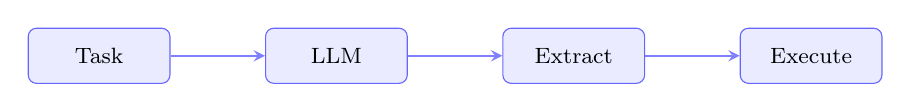
\begin{tikzpicture}[
                node distance=1.2cm,
                box/.style={rectangle, draw=blue!60, rounded corners=3pt, minimum width=1.8cm, minimum height=0.7cm, align=center, fill=blue!8, font=\footnotesize},
                arrow/.style={-stealth, thick, blue!50}
            ]
            \node[box] (input) {Task};
            \node[box, right=of input] (llm) {LLM};
            \node[box, right=of llm] (extract) {Extract};
            \node[box, right=of extract] (exec) {Execute};

            \draw[arrow] (input) -- (llm);
            \draw[arrow] (llm) -- (extract);
            \draw[arrow] (extract) -- (exec);
        \end{tikzpicture}%
    }
    \caption{Naive baseline: single-pass generation}
    \label{fig:naive-arch}
\end{figure}

This approach serves as a control condition, measuring what the LLM can achieve without architectural support.

%==============================================================================
\subsection{Single-Agent Pipeline}
\label{subsec:single-agent}

The single-agent approach introduces structured multi-phase reasoning using LangGraph~\cite{langgraph2024}, while maintaining a unified agent identity. The pipeline consists of five phases with an iterative refinement loop.

\begin{figure}[htbp]
    \centering
    \resizebox{0.9\columnwidth}{!}{%
        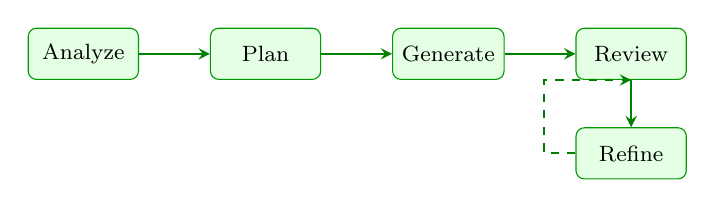
\begin{tikzpicture}[
                node distance=0.9cm,
                phase/.style={rectangle, draw=green!60!black, rounded corners=3pt, minimum width=1.4cm, minimum height=0.65cm, align=center, fill=green!10, font=\footnotesize},
                arrow/.style={-stealth, thick, green!50!black}
            ]
            \node[phase] (analysis) {Analyze};
            \node[phase, right=of analysis] (plan) {Plan};
            \node[phase, right=of plan] (gen) {Generate};
            \node[phase, right=of gen] (review) {Review};
            \node[phase, below=0.6cm of review] (refine) {Refine};

            \draw[arrow] (analysis) -- (plan);
            \draw[arrow] (plan) -- (gen);
            \draw[arrow] (gen) -- (review);
            \draw[arrow] (review) -- (refine);
            \draw[arrow, dashed] (refine.west) -- ++(-0.4,0) |- (review.south);
        \end{tikzpicture}%
    }
    \caption{Single-agent pipeline with refinement loop (max 3 iterations)}
    \label{fig:single-agent-arch}
\end{figure}

\paragraph{Phase 1: Analysis.}
Extracts structured understanding from the task specification without proposing solutions: required behavior, input/output types, constraints, edge cases, ambiguities, and common pitfalls. The prompt explicitly forbids code generation.

\paragraph{Phase 2: Planning.}
Formulates an implementation strategy based on the analysis: algorithmic approach, step-by-step implementation sequence, edge case handling, data structures, and complexity analysis (time and space).

\paragraph{Phase 3: Generation.}
Synthesizes Python code guided by the accumulated context. The prompt enforces exact signature matching, no explanatory text, and comprehensive edge case handling. A robust parser extracts code from the LLM output.

\paragraph{Phase 4: Review.}
Evaluates the generated code through execution in an isolated namespace and static analysis via Radon~\cite{radon2024}. The review distinguishes between correctness issues (which trigger refinement) and quality issues (which do not).

\paragraph{Phase 5: Refinement.}
When correctness issues are found, generates improved code based on review feedback. The loop terminates when correct or after 3 iterations. Priorities: correctness first, then edge cases, then quality.

%==============================================================================
\subsection{Multi-Agent System}
\label{subsec:multi-agent}

The multi-agent approach distributes responsibilities across three specialized agents, following the sequential chain architecture. Each agent has a distinct identity and internal reasoning pipeline.

\begin{figure}[htbp]
    \centering
    \resizebox{\columnwidth}{!}{%
        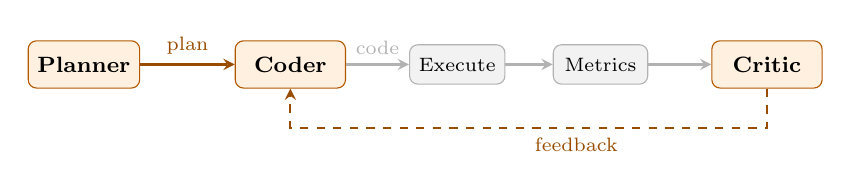
\begin{tikzpicture}[
                node distance=0.8cm,
                agent/.style={rectangle, draw=orange!70!black, rounded corners=3pt, minimum width=1.4cm, minimum height=0.6cm, align=center, fill=orange!12, font=\footnotesize\bfseries},
                process/.style={rectangle, draw=gray!60, rounded corners=3pt, minimum width=1.2cm, minimum height=0.5cm, align=center, fill=gray!10, font=\scriptsize},
                arrow/.style={-stealth, thick, orange!60!black},
                grayarrow/.style={-stealth, thick, gray!60}
            ]
            % Planner phase
            \node[agent] (planner) {Planner};

            % Coder-Critic loop
            \node[agent, right=1.2cm of planner] (coder) {Coder};
            \node[process, right=0.8cm of coder] (exec) {Execute};
            \node[process, right=0.6cm of exec] (metrics) {Metrics};
            \node[agent, right=0.8cm of metrics] (critic) {Critic};

            % Arrows
            \draw[arrow] (planner) -- node[above, font=\scriptsize] {plan} (coder);
            \draw[grayarrow] (coder) -- node[above, font=\scriptsize] {code} (exec);
            \draw[grayarrow] (exec) -- (metrics);
            \draw[grayarrow] (metrics) -- (critic);
            \draw[arrow, dashed] (critic.south) -- ++(0,-0.5) -| node[below, pos=0.2, font=\scriptsize] {feedback} (coder.south);
        \end{tikzpicture}%
    }
    \caption{Multi-agent orchestration: Planner runs once, then Coder-Critic loop iterates until correct or max iterations}
    \label{fig:multi-agent-arch}
\end{figure}

\subsubsection{Planner Agent}


The Planner is implemented as a \emph{multi-node planning agent} in LangGraph~\cite{langgraph2024}, with each node realized as a class in \texttt{planner/nodes/}. This modularization enables phase-level observability, targeted refinement, and explicit state tracking. The planner transforms a raw user request into a structured, machine-consumable plan (JSON) that serves as the contract between planning and coding, with a quality gate to prevent low-quality plans from propagating downstream.

Concretely, the Planner graph consists of six nodes:

\begin{enumerate}
    \item \textbf{Intent Analysis}: Extracts the core intent, task type, domain context, success metrics, and assumptions.
    \item \textbf{Requirements Engineering}: Produces testable functional and non-functional requirements, constraints, and edge cases.
    \item \textbf{Architecture Design}: Decomposes the solution into components, selects patterns and data structures, and outlines algorithms with complexity notes.
    \item \textbf{Implementation Planning}: Produces step-by-step coding instructions, validation rules, and representative test cases.
    \item \textbf{Quality Review}: Scores plan completeness (0--10), enumerates issues and improvements, and sets an approval flag; we require a threshold of $\geq 8$ to proceed.
    \item \textbf{Consolidation}: Assembles a unified final plan artifact for the downstream Coder agent.
\end{enumerate}

The Planner maintains an explicit state object containing each phase output (intent, requirements, architecture, implementation plan, and quality review), as well as metadata such as iteration count and accumulated errors. If the plan is not approved (quality score is below threshold), a bounded refinement loop routes feedback back to the \emph{architecture} node (rather than re-running intent/requirements), for up to two re-planning iterations, after which the system emits a best-effort consolidated plan.

\subsubsection{Coder Agent}


The Coder agent, structured in \texttt{coder/} and its \texttt{nodes/} submodule, implements a six-phase, stateful pipeline that converts plans into executable code with strict plan and signature adherence, supports iterative refinement via critic feedback, enables modular ablations and advanced reasoning backends, and incorporates robust error handling for resilience against planning or LLM failures.

\begin{enumerate}
    \item \textbf{Input Validation}: Validates function signature syntax (regex-based checks for \texttt{def}, parentheses, colon) and plan structure completeness, terminating early if critical requirements are missing.
    \item \textbf{Edge Case Analysis}: Extracts type hints from the signature via regex parsing and identifies type-specific boundary conditions (empty collections, zero/negative numerics, null strings) informed by the implementation plan.
    \item \textbf{Chain-of-Thought Generation}: Produces step-by-step reasoning that decomposes the problem into atomic steps, references identified edge cases, and plans algorithmic approach, incorporating feedback from previous iterations if refinement is active.
    \item \textbf{Code Generation}: Synthesizes Python code by accumulating context from all prior phases (signature, plan, edge cases, CoT reasoning) plus any critic feedback and execution summaries from previous iterations.
    \item \textbf{Code Validation}: Performs syntax validation via AST parsing and basic logic checks (infinite loop heuristics, unreachable code detection); accepts code with warnings but rejects on syntax errors.
    \item \textbf{Code Optimization}: Applies LLM-based refinement to improve variable naming, algorithmic efficiency, and adherence to PEP 8 style conventions; falls back to validated code if optimization fails.
\end{enumerate}

\subsubsection{Critic Agent}


The Critic agent, organized in \texttt{critic/} and its \texttt{nodes/} submodule, performs a four-phase, node-based review process with a shared state that tracks issues, scores, and structured feedback, enabling extensible validation criteria and clearly separating correctness from quality to guide systematic code refinement.

\begin{enumerate}
    \item \textbf{Input Validation}: Verifies presence of required artifacts (code, plan, signature) and halts if prerequisites are missing.
    \item \textbf{Correctness Analysis}: Evaluates functional correctness by cross-referencing code logic against plan requirements, interpreting execution error traces when available, and validating constraint satisfaction (time/space complexity, edge case handling).
    \item \textbf{Quality Review}: Assesses maintainability via static metrics (cyclomatic complexity, maintainability index from Radon), code structure clarity, and adherence to coding standards.
    \item \textbf{Feedback Synthesis}: Consolidates correctness and quality analyses into prioritized, actionable feedback for the Coder, explicitly prioritizing correctness issues over stylistic concerns to guide refinement effectively.
\end{enumerate}

\subsubsection{Orchestration}


The master workflow, defined at the orchestration level, coordinates the agents by passing explicit state objects between them: (1) Planner creates the implementation plan; (2) Coder generates code; (3) code is executed and metrics computed; (4) Critic reviews and provides feedback; (5) if the Critic identifies issues, Coder regenerates with feedback. The loop continues until the Critic approves the code or maximum iterations (default: 3) are reached. This design ensures traceability, reproducibility, and ease of extension for future research.

%==============================================================================
\subsection{Shared Infrastructure}
\label{subsec:infrastructure}

All three approaches share common components ensuring fair comparison:

\begin{itemize}
    \item \textbf{LLM Runtime}: Ollama interface with 8192-token context, 4096-token output limit, and automatic retry with backoff.
    \item \textbf{Code Extraction}: Parser handling markdown blocks (\verb|```python|), generic blocks, and raw functions; validates syntax via AST.
    \item \textbf{Execution}: Isolated namespace with captured stdout/stderr, exception handling, and function extraction verification.
    \item \textbf{Quality Metrics}: Radon-based static analysis computing Maintainability Index (0--100), Cyclomatic Complexity, LOC, and Halstead metrics.
\end{itemize}


% experiments section (imported from external file)
\input{experiments}

% conclusion section (imported from external file)
\section{Conclusion}
We presented a systematic comparison of three architectural approaches for LLM-based code generation, across 25 programming tasks.

The Naive and Multi-Agent architectures achieved identical overall functional correctness (77.6\%), yet their performance profiles differ substantially.
The Multi-Agent system justifies its computational costs in reasoning-intensive domains (Logic +10.8pp, DSA +9.4pp) where systematic planning yields a clear advantage.
In contrast, for simple pattern-matching, agentic coordination introduces unnecessary overhead that degrades performance compared to the Naive baseline. \\
Although Naive unexpectedly outperforms on Hard tasks, likely avoiding the over-refinement pitfalls of complex pipelines, our code quality analysis reveals that the Multi-Agent
approach produces more modular solutions, preserving maintainability despite increased solution complexity.

These findings suggest adaptive architecture selection: Naive for rapid prototyping, string manipulation, and known hard problems; Single-Agent for general-purpose development with
systematic edge case checking; Multi-Agent for algorithmic reasoning, constraint satisfaction, and production-quality requirements in complex domains. \\

\textbf{Limitations}: Our study is limited to 25 tasks and three model families. Future work should evaluate on larger benchmarks (APPS, CodeContests), investigate optimal refinement iteration counts,
explore heterogeneous multi-agent configurations, and develop adaptive routing mechanisms to select architectures based on task characteristics.

\bibliography{custom}

\end{document}
